\section{Release cycle management}

\textbf{Activity}

\begin{tabular}{p{7cm} p{5cm}}
    \vspace{0pt} 
    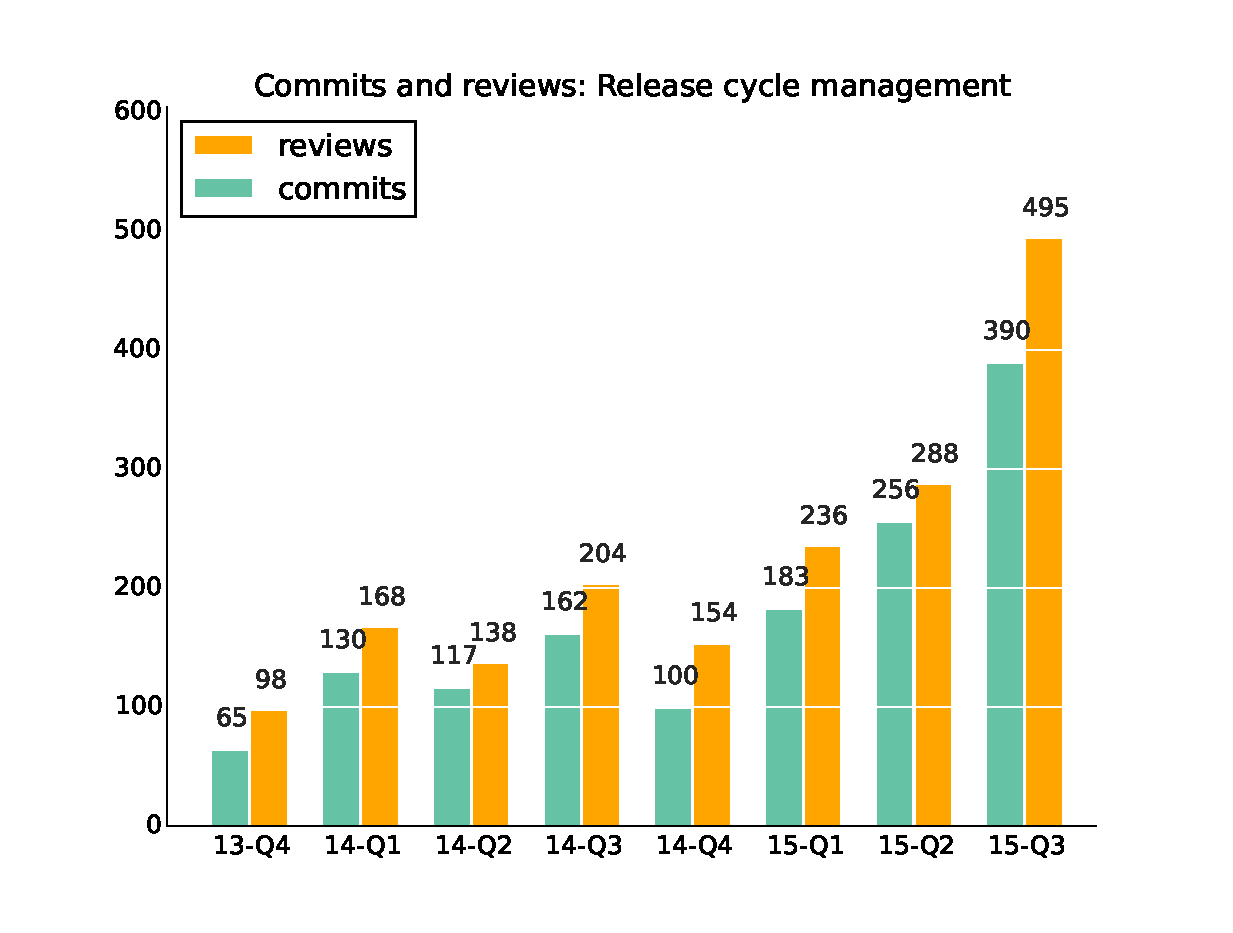
\includegraphics[scale=.35]{figs/commitsReleasecyclemanagement.eps}
    & 
    \vspace{0pt}
    \begin{tabular}{l|r|r|}%
    \bfseries Period & \bfseries Commits & \bfseries Reviews % specify table head
    \csvreader[head to column names]{data/commitsReleasecyclemanagement.csv}{}% use head of csv as column names
    {\\\labels & \commits & \submitted}
    \end{tabular}
\end{tabular}

\begin{tabular}{p{7cm} p{5cm}}
    \vspace{0pt} 
    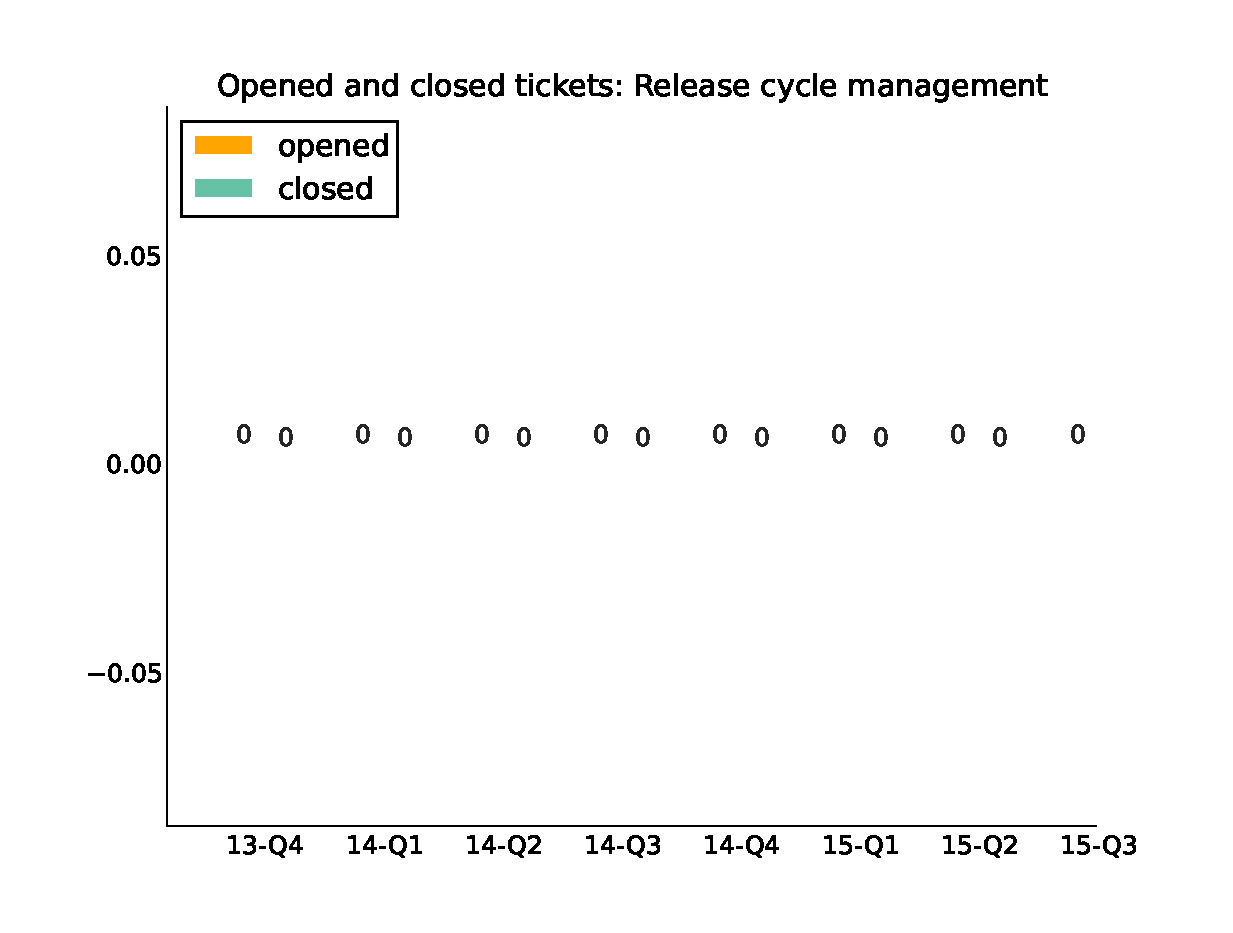
\includegraphics[scale=.35]{figs/closedReleasecyclemanagement.eps}
    & 
    \vspace{0pt}
    \begin{tabular}{l|r|r|}%
\bfseries Period & \bfseries Closed & \bfseries Opened
    \csvreader[head to column names]{data/closedReleasecyclemanagement.csv}{}% use head of csv as column names
    {\\\labels & \closed & \opened}
    \end{tabular}
\end{tabular}

\begin{tabular}{p{7cm} p{5cm}}
    \vspace{0pt} 
    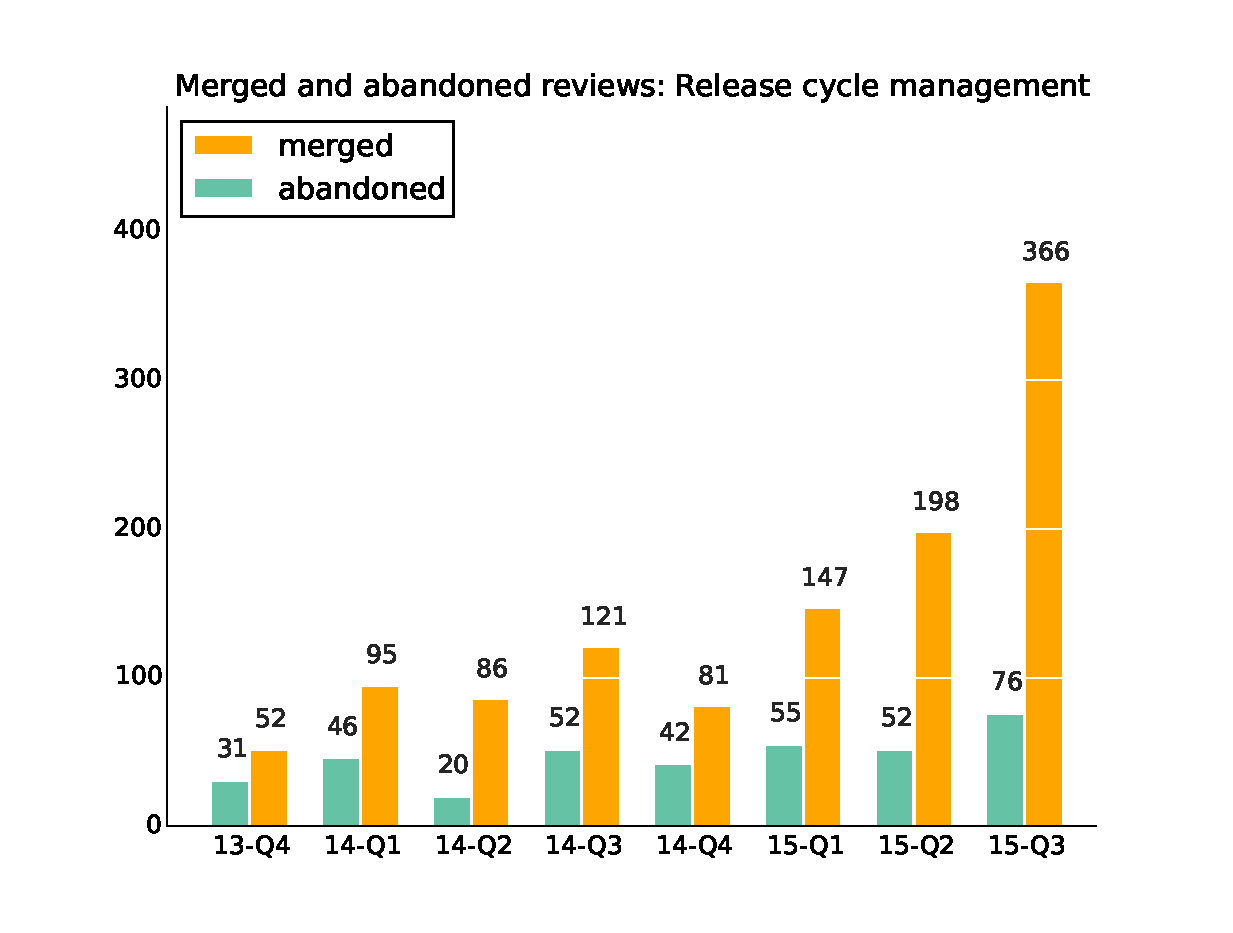
\includegraphics[scale=.35]{figs/submitted_reviewsReleasecyclemanagement.eps}
    & 
    \vspace{0pt}
    \begin{tabular}{l|r|r|}%
    \bfseries Period & \bfseries Merged & \bfseries Abandoned % specify table head
    \csvreader[head to column names]{data/submitted_reviewsReleasecyclemanagement.csv}{}% use head of csv as column names
    {\\\labels & \merged & \abandoned}
    \end{tabular}
\end{tabular}

\textbf{Community}

\begin{tabular}{p{7cm} p{5cm}}
    \vspace{0pt} 
    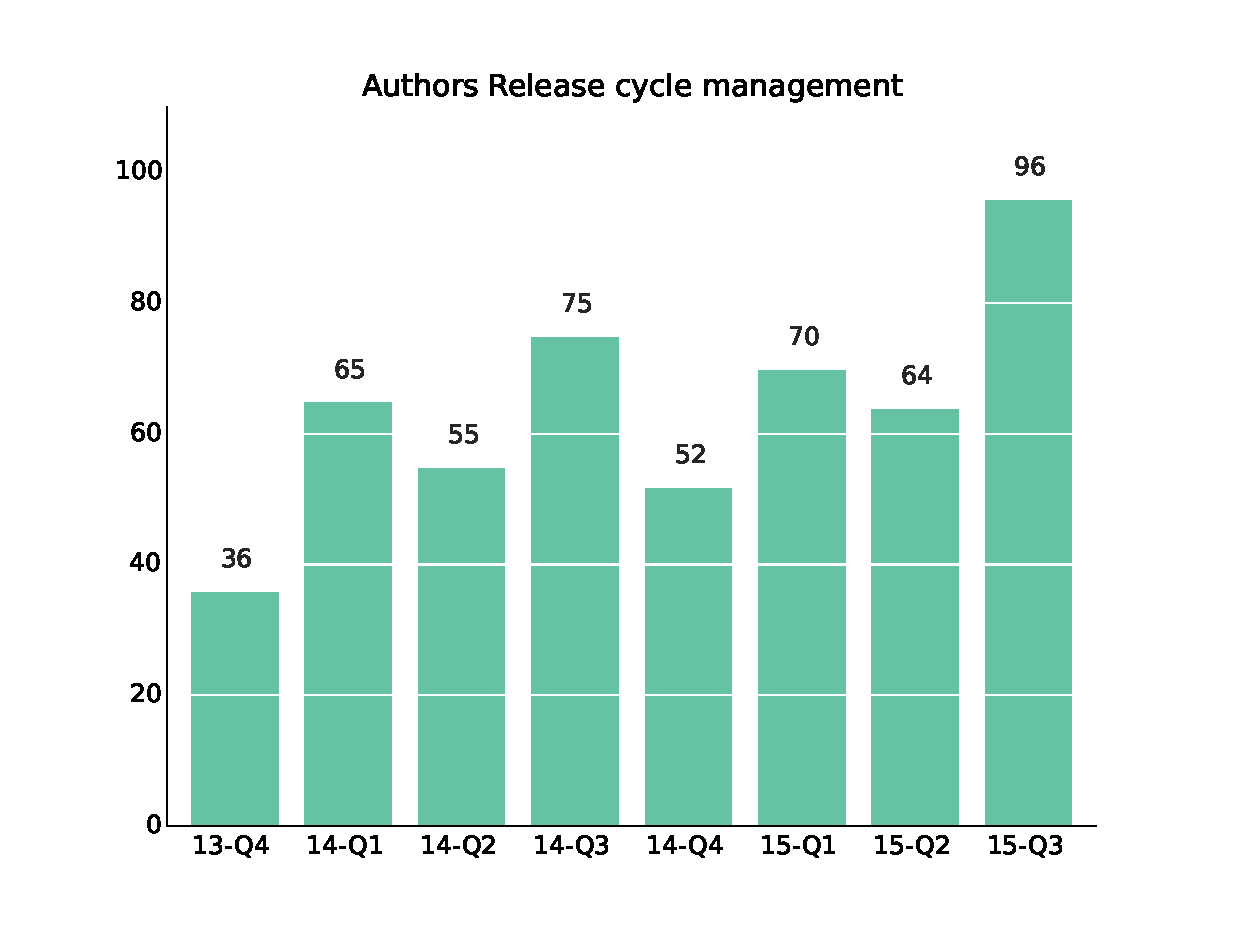
\includegraphics[scale=.35]{figs/authorsReleasecyclemanagement.eps}
    & 
    \vspace{0pt}
    \begin{tabular}{l|l}%
    \bfseries Period & \bfseries Authors % specify table head
    \csvreader[head to column names]{data/authorsReleasecyclemanagement.csv}{}% use head of csv as column names
    {\\\labels & \authors}
    \end{tabular}
\end{tabular}

\begin{tabular}{p{7cm} p{5cm}}
    \vspace{0pt}
\begin{tabular}{l|l}%
    \bfseries Commit (s) & \bfseries Author % specify table head
    \csvreader[head to column names]{data/scm_top_authors_project_Releasecyclemanagement.csv}{}% use head of csv as column names
    {\\\hline\csvcoli&\csvcolii}% specify your coloumns here
\end{tabular}
&
\vspace{0pt}
\begin{tabular}{l|l}%
    \bfseries Commit (s) & \bfseries Organizations % specify table head
    \csvreader[head to column names]{data/scm_top_companies_project_Releasecyclemanagement.csv}{}% use head of csv as column names
    {\\\hline\csvcoli&\csvcolii}% specify your coloumns here
\end{tabular}
\end {tabular}

\textbf{Process}

\begin{tabular}{p{7cm} p{5cm}}
    \vspace{0pt} 
    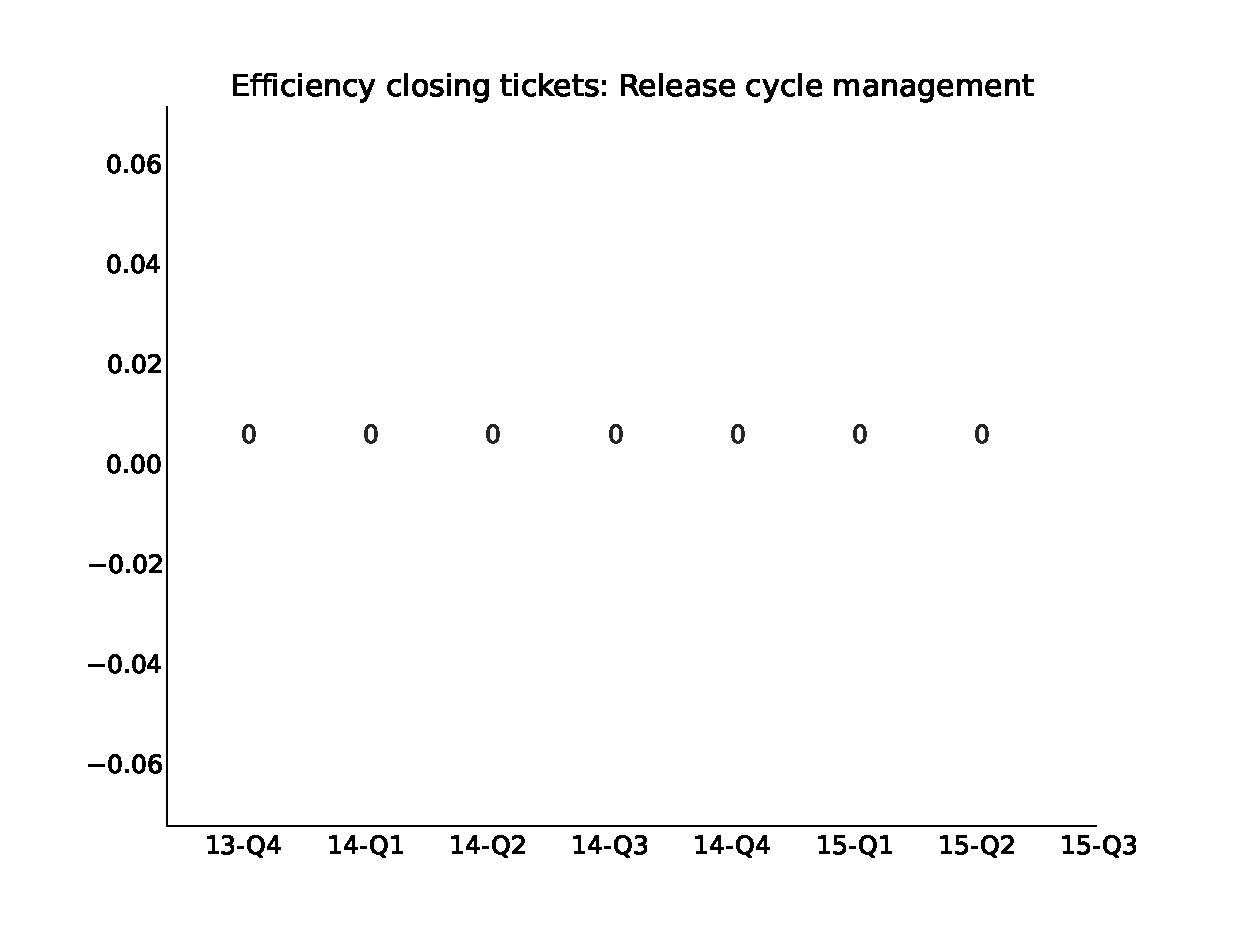
\includegraphics[scale=.35]{figs/bmiReleasecyclemanagement.eps}
    & 
    \vspace{0pt}
    \begin{tabular}{l|l}%
    \bfseries Period & \bfseries Closed/Opened % specify table head
    \csvreader[head to column names]{data/bmiReleasecyclemanagement.csv}{}% use head of csv as column names
    {\\\labels & \bmi}
    \end{tabular}
\end{tabular}

\begin{tabular}{p{7cm} p{5cm}}
    \vspace{0pt} 
    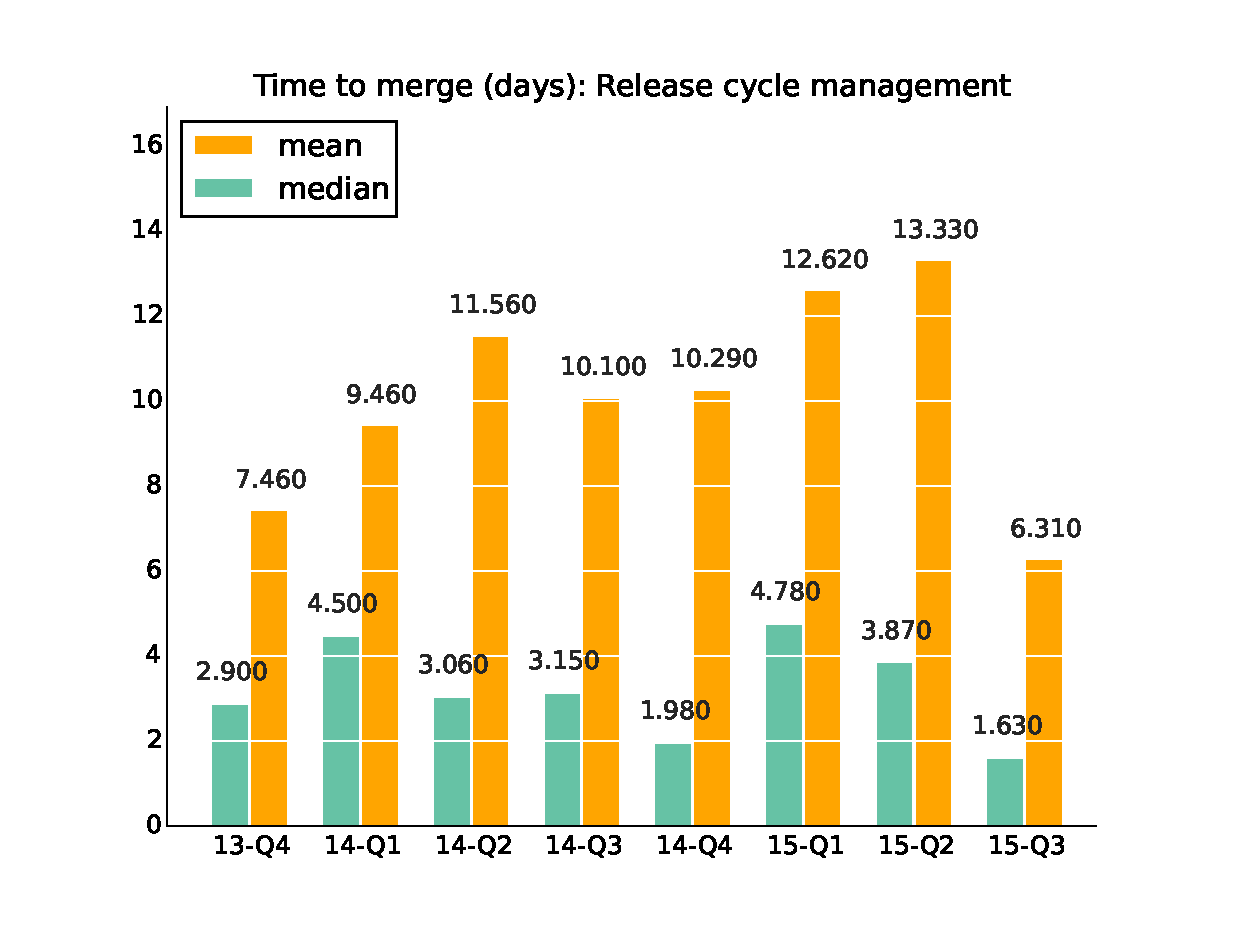
\includegraphics[scale=.35]{figs/timetoreview_medianReleasecyclemanagement.eps}
    & 
    \vspace{0pt}
    \begin{tabular}{l|r|r|}%
    \bfseries Period & \bfseries Median & \bfseries Mean % specify table head
    \csvreader[head to column names]{data/timetoreview_medianReleasecyclemanagement.csv}{}% use head of csv as column names
    {\\\labels & \mediantime & \meantime}
    \end{tabular}
\end{tabular}

